%%%%%%%%%%%%%%%%%%%%%%%%%%%%%%%%%%%%%%%%%%%%%%%%%%%%%%%%%%%%%%%%%%%%%%%%%%%%%%%%
\documentclass[11pt]{article}

\usepackage[authoryear]{natbib}
\usepackage[top=2.5cm,bottom=2.5cm,left=2.5cm,right=2.5cm]{geometry}
\usepackage{color}
\usepackage{chemarr}
\usepackage{amssymb}
\usepackage{graphicx}
\usepackage{textcomp} 
\usepackage[gen]{eurosym}
\usepackage{amsmath}
\usepackage[margin=1.5cm]{caption}
\usepackage{amsmath,mathtools}
\usepackage{subcaption}
%\usepackage{ulem}
\usepackage[normalem]{ulem}
%\setlength{\belowcaptionskip}{-5pt}
%\setlength{\abovecaptionskip}{-8pt}
\usepackage{enumitem}

%\usepackage[autolinebreaks,useliterate]{mcode}
\usepackage[usenames, dvipsnames]{xcolor}
\colorlet{shadecolor}{gray!5}
\usepackage{listings}
\lstset{ 
	language=R,                     % the language of the code
	basicstyle=\scriptsize\ttfamily, 	  % the size of the fonts
	numbers=left,                   % where to put the line-numbers
	numberstyle=\tiny\color{Blue},  % the style that is used for the line-numbers
	stepnumber=1,                   % the step between two line-numbers.
	numbersep=5pt,                  % how far the line-numbers are from the code
	backgroundcolor=\color{shadecolor},  % choose the background color.
	showspaces=false,               % show spaces adding particular underscores
	showstringspaces=false,         % underline spaces within strings
	showtabs=false,                 % show tabs within strings adding particular underscores
	frame=tb,                   	  % adds a frame around the code
	rulecolor=\color{Black},        % if not set, the frame-color may be changed on line-breaks within not-black text (e.g. commens (green here))
	tabsize=2,                      % sets default tabsize to 2 spaces
	captionpos=b,                   % sets the caption-position to bottom
	breaklines=true,                % sets automatic line breaking
	breakatwhitespace=false,        % sets if automatic breaks should only happen at whitespace
	keywordstyle=\color{RoyalBlue}, % keyword style
	commentstyle=\color{OliveGreen},% comment style
	stringstyle=\color{ForestGreen} % string literal style
}

\newcommand{\nrtodo}[1]{{\color{blue} NR: #1}}

%%%%%%%%%%%%%%%%%%%%%%%%%%%%%%%%%%%%%%%%%%%%%%%%%%%%%%%%%%%%%%%%%%%%%%%%%%%%%%%%
\title{\textbf{Comparing BC mixing state from CAMChem to SP2 measurements}}
\author{Yinrui Li}
\date{}


%\maketitle


\begin{document}
	\maketitle
	%%%%%%%%%%%%%%%%%%%%%%%%%%%%%%%%%%%%%%%%%%%%%%%%%%%%%%%%%%%%%%%%%%%%%%%%%%%%%%%%
	
	
	
	\section{SP2 Measurement} 
	
	The SP2 instrument measures the BC particle cores over a calibrated volume equivalent diameter (VED) range of 55--400~nm, which is unlikely to represent the total
	ambient number and mass concentrations of BC particles \citep{Reddington2013}. In order to compare CAMChem model simulated BC with observations, we estimated the mass fraction of modeled BC in the size range corresponding to SP2 measurement. SP2 number-detection efficiency at sea level pressure is reported to be 100$\%$ for BC above 90~nm VED \citep{Schwarz2010a}, so following Reddington et al., 2013, we use 90~nm--400~nm as the efficient diameter range of SP2 measurement in this study.

	\section{Estimating the mean BC core diameter in primary carbon mode and in accumulation mode} 
	
	A 4-mode version of the modal aerosol model (MAM4) is applied in
	CAMChem1.2.2. BC is emitted to the primary carbon mode, and then is
	transferred to the accumulation mode by condensation of
	$\rm{H_2SO_4}$, $\rm{NH_3}$ and $\rm{SOA}$ and by coagulation \citep{Liu2012}. In primary carbon mode, particles consist of externally
	mixed BC and OC, whereas in accumulation mode, particles consist of
	internally mixed BC and non-BC material. The version of 4 lognormal modes (MAM4) assumes that the particle size distributions in each mode has a fixed geometric standard deviation and a changeable geometric mean diameter.
	
	
	The geometric mean diameter of BC core is interpreted as:
	\begin{align*}
	d = (d_{\text{mixed}}^3 \times f_{\text{BC}})^\frac{1}{3}, 
	\end{align*}
	where $d$ is the geometric mean diameter of BC core,
	$d_{\text{mixed}}$ is the geometric mean diameter of internally mixed particles
	(\textbf{extracted from model}), and $f_{\text{BC}}$ is the volume
	fraction of BC in accumulation mode. For the following estimation of volume fraction within SP2 measurement size range, we refer to the geometric mean diameter of BC particles as its core diameter.
	
	\section{Compute Volume Fraction within size range for a Lognormal Distribution}
	The CDF of lognormal number distribution of the BC cores in the diameter range between $d_{1}$ and
	$d_{2}$ is:
	\begin{align*}
	N(d_{1}, d_{2}) = \frac{1}{\text{ln}\sigma_{\text{g}}\sqrt{2\pi}}\int_{d_{1}}^{d_{2}}e^-\frac{(\text{ln}d - \text{ln}d_{\rm g})^2}{2\text{ln}^2\sigma_{\text{g}}}\text{d}(\text{ln}d),
	\end{align*}
	where $d_{\rm g}$ is the geometric mean diameter of the BC core distribution (extracted from the model, varying temporally and spatially). 
	
	The third moment of the lognormal distribution of BC core between 90 and 400~nm (proportional to the volume of BC cores whose diameter is within that size range) is:
	\begin{align*}
	V(d_{1}, d_{2}) &= \frac{1}{\text{ln}\sigma_{\text{g}}\sqrt{2\pi}}\int_{d_{1}}^{d_{2}}d^3e^-\frac{(\text{ln}d - \text{ln}d_{\rm g})^2}{2\text{ln}^2\sigma_{\text{g}}}\text{d}(\text{ln}d)  \\
	&=\frac{e^{\frac{k^2}{2}\text{ln}^2\sigma_{\rm g}+k\text{ln}d_{\rm g}}}{\text{ln}\sigma_{\text{g}}\sqrt{2\pi}}\int_{d_{1}}^{d_{2}}d^3e^-\frac{(\text{ln}d - \text{ln}d_{\text{gv}})^2}{2\text{ln}^2\sigma_{\text{g}}}\text{d}(\text{ln}d),
	\end{align*}
	where the geometric mean diameter of BC volume is represented as $\text{ln}d_{\text{gv}}
	= \text{ln}d_{\text{g}} + 3\text{ln}\sigma_{\text{g}}$
	
	So the mass fraction of the BC cores in the size range between $d_{1}$ and $d_{2}$ (in each mode) is derived as:
	
	\begin{align*}
	F(d_{1}, d_{2}) &= \frac{\frac{1}{\text{ln}\sigma_{\text{g}}\sqrt{2\pi}}\int_{d_{1}}^{d_{2}}d^3e^-\frac{(\text{ln}d - \text{ln}d_{\rm g})^2}{2\text{ln}^2\sigma_{\text{g}}}\text{d}(\text{ln}d)}
	{\frac{1}{\text{ln}\sigma_{\text{g}}\sqrt{2\pi}}\int_{-\infty}^{+\infty}d^3e^-\frac{(\text{ln}d - \text{ln}d_{\rm g})^2}{2\text{ln}^2\sigma_{\text{g}}}\text{d}(\text{ln}d)}  \\
	&=\frac{\frac{e^{\frac{k^2}{2}ln^2\sigma_{\rm g}+k\text{ln}d_{\rm g}}}{\text{ln}\sigma_{\text{g}}\sqrt{2\pi}}\int_{d_{1}}^{d_{2}}e^-\frac{(\text{ln}d - \text{ln}d_{\text{gv}})^2}{2\text{ln}^2\sigma_{\text{g}}}\text{d}(\text{ln}d)}{\frac{e^{\frac{k^2}{2}ln^2\sigma_{\rm g}+k\text{ln}d_{\rm g}}}{\text{ln}\sigma_{\text{g}}\sqrt{2\pi}}\int_{-\infty}^{+\infty}e^-\frac{(\text{ln}d - \text{ln}d_{\text{gv}})^2}{2\text{ln}^2\sigma_{\text{g}}}\text{d}(\text{ln}d)}\\
	&=\frac{1}{\text{ln}\sigma_{\text{g}}\sqrt{2\pi}}\int_{d_{1}}^{d_{2}}e^-\frac{(\text{ln}d - \text{ln}d_{\text{gv}})^2}{2\text{ln}^2\sigma_{\text{g}}}\text{d}(\text{ln}d) \\
	&=\frac{1}{2}[\text{erf}(\frac{\text{ln}d_{2} - \text{ln}d_{\text{gv}}}{\sqrt{2}\text{ln}\sigma_{\rm g}})-\text{erf}(\frac{\text{ln}d_{1} - \text{ln}d_{\text{gv}}}{\sqrt{2}\text{ln}\sigma_{\rm g}})],
	\end{align*}
	
	The above mass fraction for primary carbon mode ($F_{\text{pc}}(d_{1}, d_{2})$) and for accumulation mode ($F_{\text{accu}}(d_{1}, d_{2}$) do not add up to 1:
	\[F_{\text{accu}}(d_{1}, d_{2}) + F_{\text{pc}}(d_{1}, d_{2}) \neq 1,\]
	
	
	
	\textbf{Within the size range (90--400~nm)}, the ratios of the mass of BC cores in each mode to the total mass of BC cores are computed as:
	\begin{align*}
	f_{\text{accu}} = \frac{F_{\text{accu}}(d_{1}, d_{2})M_{\text{accu}}}{F_{\text{accu}}(\text{d}_{1}, d_{2})M_{\text{accu}}+F_{\text{pc}}(d_{1}, d_{2})M_{\text{pc}}}\\
	f_{\text{pc}} = \frac{F_{\text{pc}}(d_{1}, d_{2})M_{\text{pc}}}{F_{\text{accu}}(d_{1}, d_{2})M_{\text{accu}}+F_{\text{pc}}(d_{1}, d_{2})M_{\text{pc}}}
	\end{align*}
	\[f_{\text{accu}} + f_{\text{pc}} = 1,\]
	
	where $f_{\text{accu}}$ is the mass fraction of BC cores in
	accumulation mode, $f_{\text{pc}}$ is the mass fraction of BC cores in
	primary carbon mode, $M_{\text{accu}}$ and $M_{\text{pc}}$ are the mass mixing ratio of BC cores
	in accumulation mode and primary carbon mode, respectively.
	
	Sketch of F and f are shown in Figure~\ref{fig_P1}, Figure~\ref{fig_P2} and Figure~\ref{fig_P3}.
	
	\begin{figure}[!h] 
		\begin{center}
			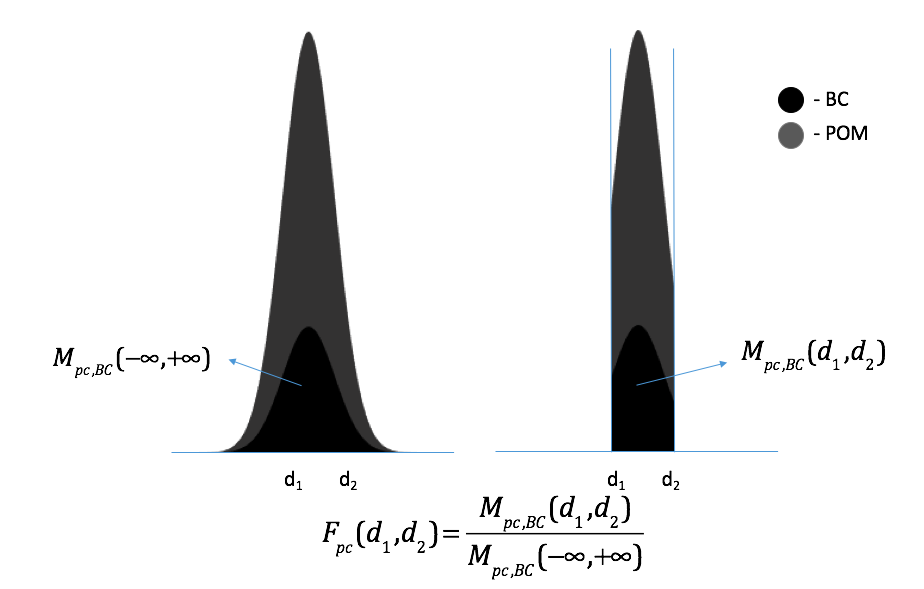
\includegraphics[width = 0.8\textwidth]{Rplot05}
			\caption[]{\label{fig_P1} BC mass fraction within the SP2 size range for primary carbon mode $F_{\text{pc}}(d_{1}, d_{2})$.}
		\end{center}
	\end{figure}
	
	\begin{figure}[!h] 
		\begin{center}
			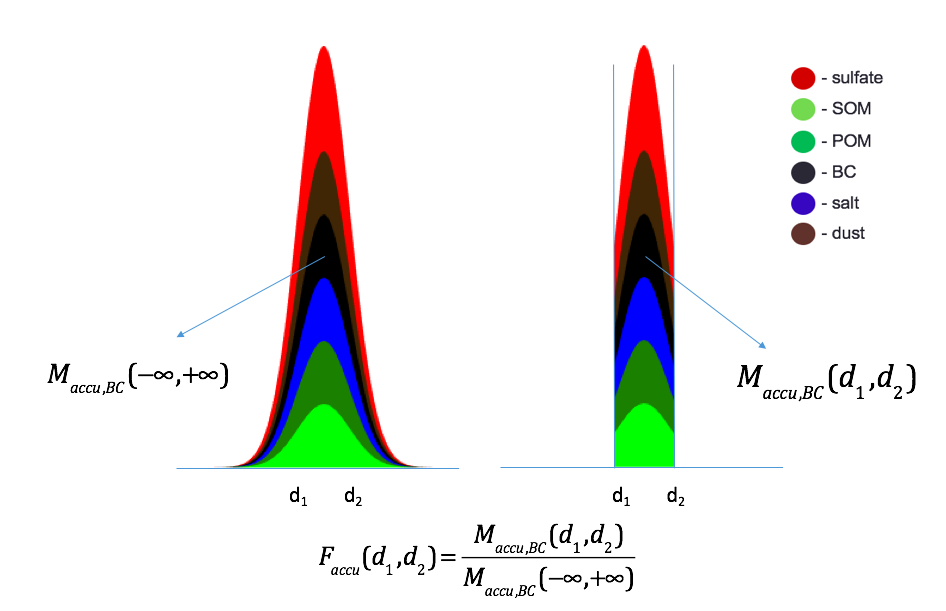
\includegraphics[width = 0.8\textwidth]{Rplot06}
			\caption[]{\label{fig_P2} BC mass fraction within the SP2 size range for accumulation mode $F_{\text{accu}}(d_{1}, d_{2})$.}
		\end{center}
	\end{figure}
	
	\begin{figure}[!h] 
		\begin{center}
			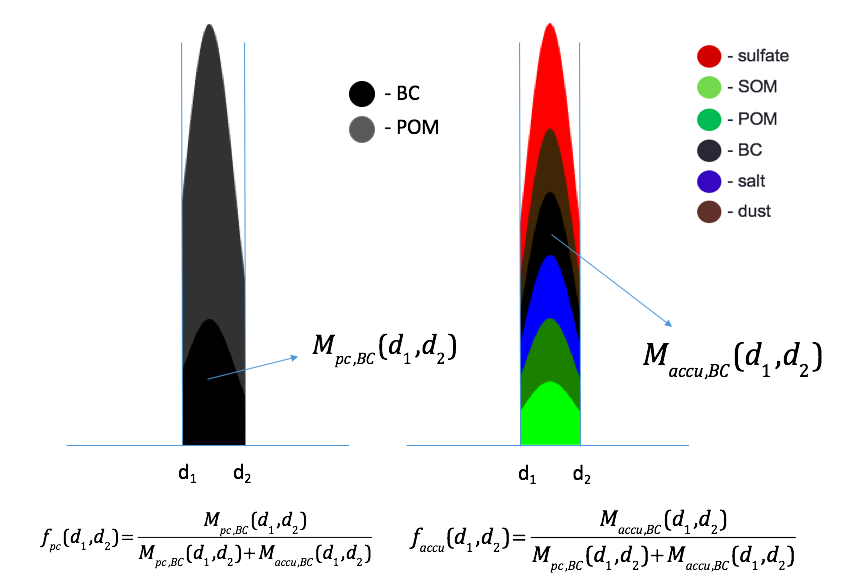
\includegraphics[width = 0.7\textwidth]{Rplot07}
			\caption[]{\label{fig_P3} The ratios of BC mass in the SP2 size range in each mode to the total BC mass in the SP2 size range, for primary carbon mode $f_{\text{pc}}(d_{1}, d_{2})$ and for accumulation mode $f_{\text{accu}}(d_{1}, d_{2})$.}
		\end{center}
	\end{figure}
	
	
	Generally, the mixing ratio of BC particles in the accumulation mode is higher ($M_{\text{accu}}$) than that in the primary carbon mode ($M_{\text{pc}}$) when it is distant from the source regions (e.g., Indian Ocean, Atlantic Ocean) (Figure~\ref{fig_P4}), primarily because black carbon will be transfered from the fresh, hydrophobic mode (primary carbon) into the aged, hydrophilic mode (accumulation) during transportation. We also observe that for some Arctic regions (e.g., Greenland), however, BC mixing ratio can be higher in the primary carbon mode than in the accumulation mode.
	
	BC mass fractions within the SP2 size range ($F_{\text{pc}}(90~\text{nm}, 400~\text{nm})$ and
	$F_{\text{accu}}(90~\rm nm, 400~\rm nm)$) are shown in Figure~\ref{fig_P5}. For primary carbon mode
	(upper panel), SP2 would be able to detect most of BC ($\textgreater$60$\%$) over the ocean and throughout the North Pole, and less of BC ($\textless$40$\%$) in regions like central Africa, Northeast Asia and Australia. For accumulation mode (lower panel), this portion is higher when it is close to the sources (e.g., South East Asia, Europe), and lower at high latitudes. We also observe that the distributions of the above mass fractions (Figure~\ref{fig_P5}) have similar pattern with the size distributions of BC cores (Figure~\ref{fig_P6}), which indicates that the low values of the mass fraction ($F_{\text{pc}}(90~\text{nm}, 400~\text{nm})$ and $F_{\text{accu}}(90~\text{nm}, 400~\text{nm}$) are highly due to the small geometric mean diameter of BC cores ($\textless$90~nm)in that region.
	\begin{figure}[!h] 
		\begin{center}
			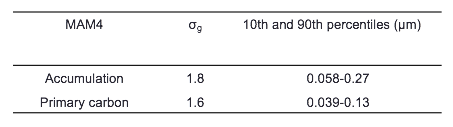
\includegraphics[width = 0.6\textwidth]{Rplot01}
			\caption[]{\label{fig_P4}BC mass mixing ratio ($M_{\rm pc}$ and $M_{\rm accu}$) in primary carbon mode (top) and in accumulation mode (bottom), for surface layer, March.}
		\end{center}
	\end{figure}
	
	\begin{figure}[!h] 
		\begin{center}
			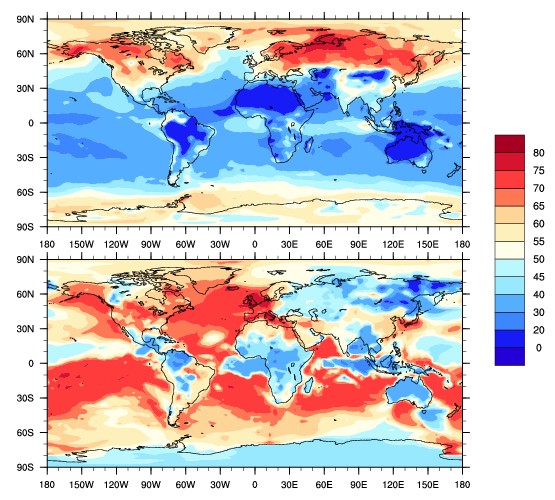
\includegraphics[width = 0.6\textwidth]{Rplot02}
			\caption[]{\label{fig_P5} BC mass fraction between 90 and 400~nm ($F_{\rm pc}$ and $F_{\rm accu}$) in primary carbon mode (top) and in accumulation mode (bottom), for surface layer, March.}
		\end{center}
	\end{figure}
	
	\begin{figure}[!h] 
		\begin{center}
			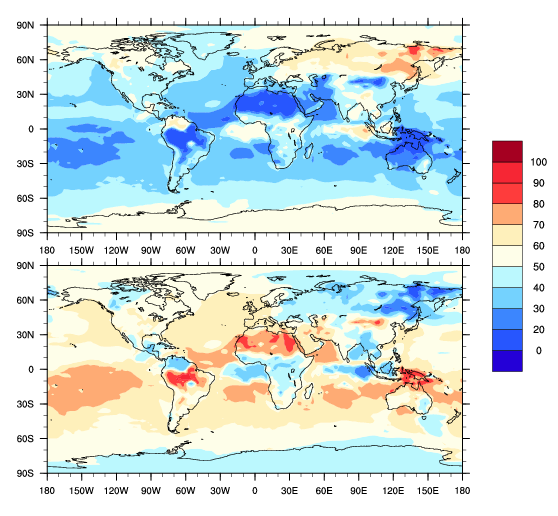
\includegraphics[width = 0.6\textwidth]{Rplot03}
			\caption[]{\label{fig_P6} Geometric mean diameter of BC core ($\mu$m) in primary carbon mode (top) and accumulation mode (bottom), for surface layer, March.}
		\end{center}
	\end{figure}
	
	
	
	The ratios of BC mixing ratio in each mode within the SP2 size range to the total BC mixing ratio within the SP2 size range ($f_{\rm pc}$ and $f_{\rm accu}$) are shown in Figure~\ref{fig_P7}, which represents the mixing states of BC particles that are captured by SP2 measurements. Most of them are internally mixed in the low and middle
	latitudes ($f_{\rm accu}\textgreater$60$\%$), and are externally mixed at high latitudes ($f_{\rm pc}\textgreater$60$\%$). The mixing state can vary spatially in the Arctic region,
	which should be taken into consideration when comparing modeled BC
	with SP2 measurements. Fractions in two panels should add up to 1.
	
	
	
	\begin{figure}[!h] 
		\begin{center}
			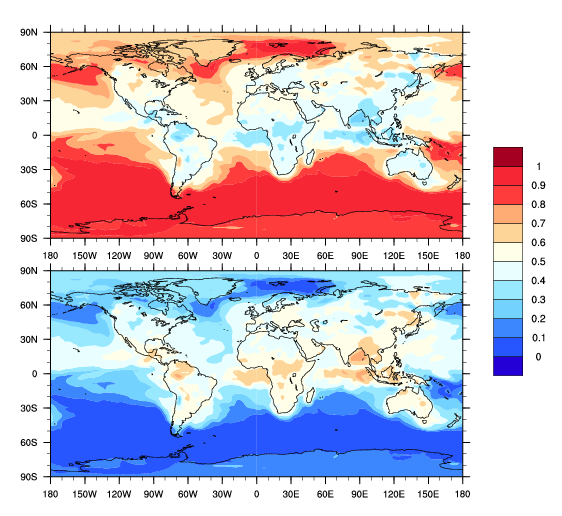
\includegraphics[width = 0.6\textwidth]{Rplot04}
			\caption[]{\label{fig_P7} Ratio of BC mixing ratio within SP2 size range to total BC mixing ratio within SP2 size range in primary carbon mode $f_{\rm pc}$ (top) and in accumulation mode $f_{\rm accu}$ (bottom), for surface layer, March.}
		\end{center}
	\end{figure}
	
	
	
	
	
	\clearpage
	
	\bibliographystyle{plain-local-srefid}
	\bibliography{refs}
	
	
	
	
	
	
	%%%%%%%%%%%%%%%%%%%%%%%%%%%%%%%%%%%%%%%%%%%%%%%%%%%%%%%%%%%%%%%%%%%%%%%%%%%%%%%%
	
	
	
\end{document}
%%%%%%%%%%%%%%%%%%%%%%%%%%%%%%%%%%%%%%%%%%%%%%%%%%%%%%%%%%%%%%%%%%%%%%%%%%%%%%%%
%%%%%%%%%%%%%%%%%%%%%%%%%%%%%%%%%%%%%%%%%%%%%%%%%%%%%%%%%%%%%%%%%%%%%%%%%%%%%%%%
